\documentclass[aps,rmp,reprint,amsmath,amssymb,graphicx,longbibliography]{revtex4-1}

\usepackage{bm}
\usepackage{graphicx}% Include figure files

\newcommand{\vq}{{\vec q}}
\newcommand{\vf}{v_{\rm F}}
\newcommand{\kf}{k_{\rm F}}
\newcommand{\Phio}{\Phi_0}
\newcommand{\tp}{t_\perp}
\newcommand{\Hca}{\mathcal{H}}
\newcommand{\vk}{{\bf k}}

\begin{document}

\title{The Quantum Internet | Towards the Singularity}

\author{Peter Rohde}
\affiliation{UTS}


\author{Other dudes}

\affiliation{Other affiliations}

\author{Tim Byrnes}
\affiliation{State Key Laboratory of Precision Spectroscopy, School of Physical and Material Sciences,
East China Normal University, Shanghai 200062, China}
\affiliation{NYU-ECNU Institute of Physics at NYU Shanghai, 3663 Zhongshan Road North, Shanghai 200062, China}
\affiliation{National Institute of Informatics, 2-1-2 Hitotsubashi, Chiyoda-ku, Tokyo 101-8430, Japan}
\affiliation{New York University Shanghai, 1555 Century Ave, Pudong, Shanghai 200122, China} 
\affiliation{Department of Physics, New York University, New York, NY 10003, USA}
 

\author{Jonathan P. Dowling}
\affiliation{Hearne Institute for Theoretical Physics, Department of Physics \& Astronomy, Louisiana State University, Baton Rouge, Louisiana 70803-4001, USA}




\date{\today{}}

\begin{abstract}
[Abstract]
\end{abstract}

%\pacs{81.05.Uw,68.37.-d,73.20-r}

\maketitle

\tableofcontents{}





\section{Foreword}
\label{foreword}

[Previous sections]





\section{Space based quantum communication}
\label{sec:space}

[TB: This introductory paragraph probably needs integrating with what is written already, such as adding section references]

One of the major hurdles that must be overcome before quantum networks to gain widespread commercial use is to span large distances between nodes.  The key technological and commercial centers of the world are spread worldwide, hence connections over intercontinental distances are necessary, with nodes separated by several thousands of kilometers. This distance is one of the major challenges facing the creation of a large-scale quantum quantum networks. The most convenient way of transmitting quantum information is using optical fibers. However, it is well-known that due to the exponential scaling of loss with distance, the upper limit is of the order of several hundred kilometers. This shortcoming has led to intense research relating to extending these distances using quantum repeaters. In a quantum repeater, one creates long-distance entanglement by joining together entangled pairs, established over multiple short-distance links, through entanglement swapping \cite{sangouard11}. Much research has been done in this direction, but such quantum repeaters remain a challenging task primarily due to the lack of a reliable quantum memory -- a medium that can store quantum information and convert it reliably between photons \cite{lvovsky2009optical,simon2010quantum,bussieres2013prospective, heshami2016quantum}. 

An alternative to optic fiber communication is using terrestrial free-space links. Particular wavelength ranges have low absorption, and it is possible to propagate photons across large distances. Impressive experimental demonstrations of teleportation with free-space entanglement by Zeilinger and co-workers \cite{ursin07,ma2012quantum,yin2013lower} over 100km have been achieved. However, extending to longer distances have been problematic.  Photon loss in free space links is affected by weather conditions and other effects, such as pollution, that degrade visibility. The Earth’s curvature provides an absolute upper limit, depending on the elevation of the source and receiver. For example, for an observer on a 30m tower, the horizon is at a distance of 20km, a relatively short distance. The observatory used in the experiments performed by the experiments of Ref. \cite{ursin07,ma2012quantum} were are at an elevation of 2393m, which allowed for the 143km transmission. 

One attractive possibility to overcome these issues is using space-based quantum communication. In this scenario, satellites orbiting the Earth would act as nodes of the quantum network, which could store, send and receive quantum information. At altitudes where satellites orbit the Earth, photon loss due to scattering is negligible, and photons can propagate across extremely long distances. The main loss in this case is caused by diffraction, due to the finite diameter of the receiver and transmitter. For example, using reasonable diameters it is in the region of 40-80 dB loss for low Earth orbit \cite{aspelmeyer2003long,liao2016ground}. Involving ground-based quantum network nodes is also not an inherent problem as 80\% of the atmosphere by mass is located within the first 12km in altitude. Ground-to-satellite and satellite-to-ground quantum communication has already been demonstrated, as will be discussed more in the next section. Such a satellite-based quantum communication system is naturally suited to various tasks, in particular quantum cryptography which does not require quantum memories. But with the addition of quantum memories the capabilities of such a quantum network could be greatly enhanced, making many of the applications listed above a possibility at the global scale. 


Naturally, such a space-based quantum network comes with enormous challenges that much be overcome before it is implemented. Creating even a short-distance quantum network is currently technologically challenging, let alone one that is loaded onto a satellite transmitting photons across distances potentially of the order of the diameter of the Earth. The cooperation of space agencies is necessary even for initial experiments. As we describe more in the next section, several recent positive results has made the technology an immediate possibility in realizing such a global level quantum network. In this section, we summarize the current technological state of the art internationally, and discuss some of the remaining major challenges.  




\begin{figure}
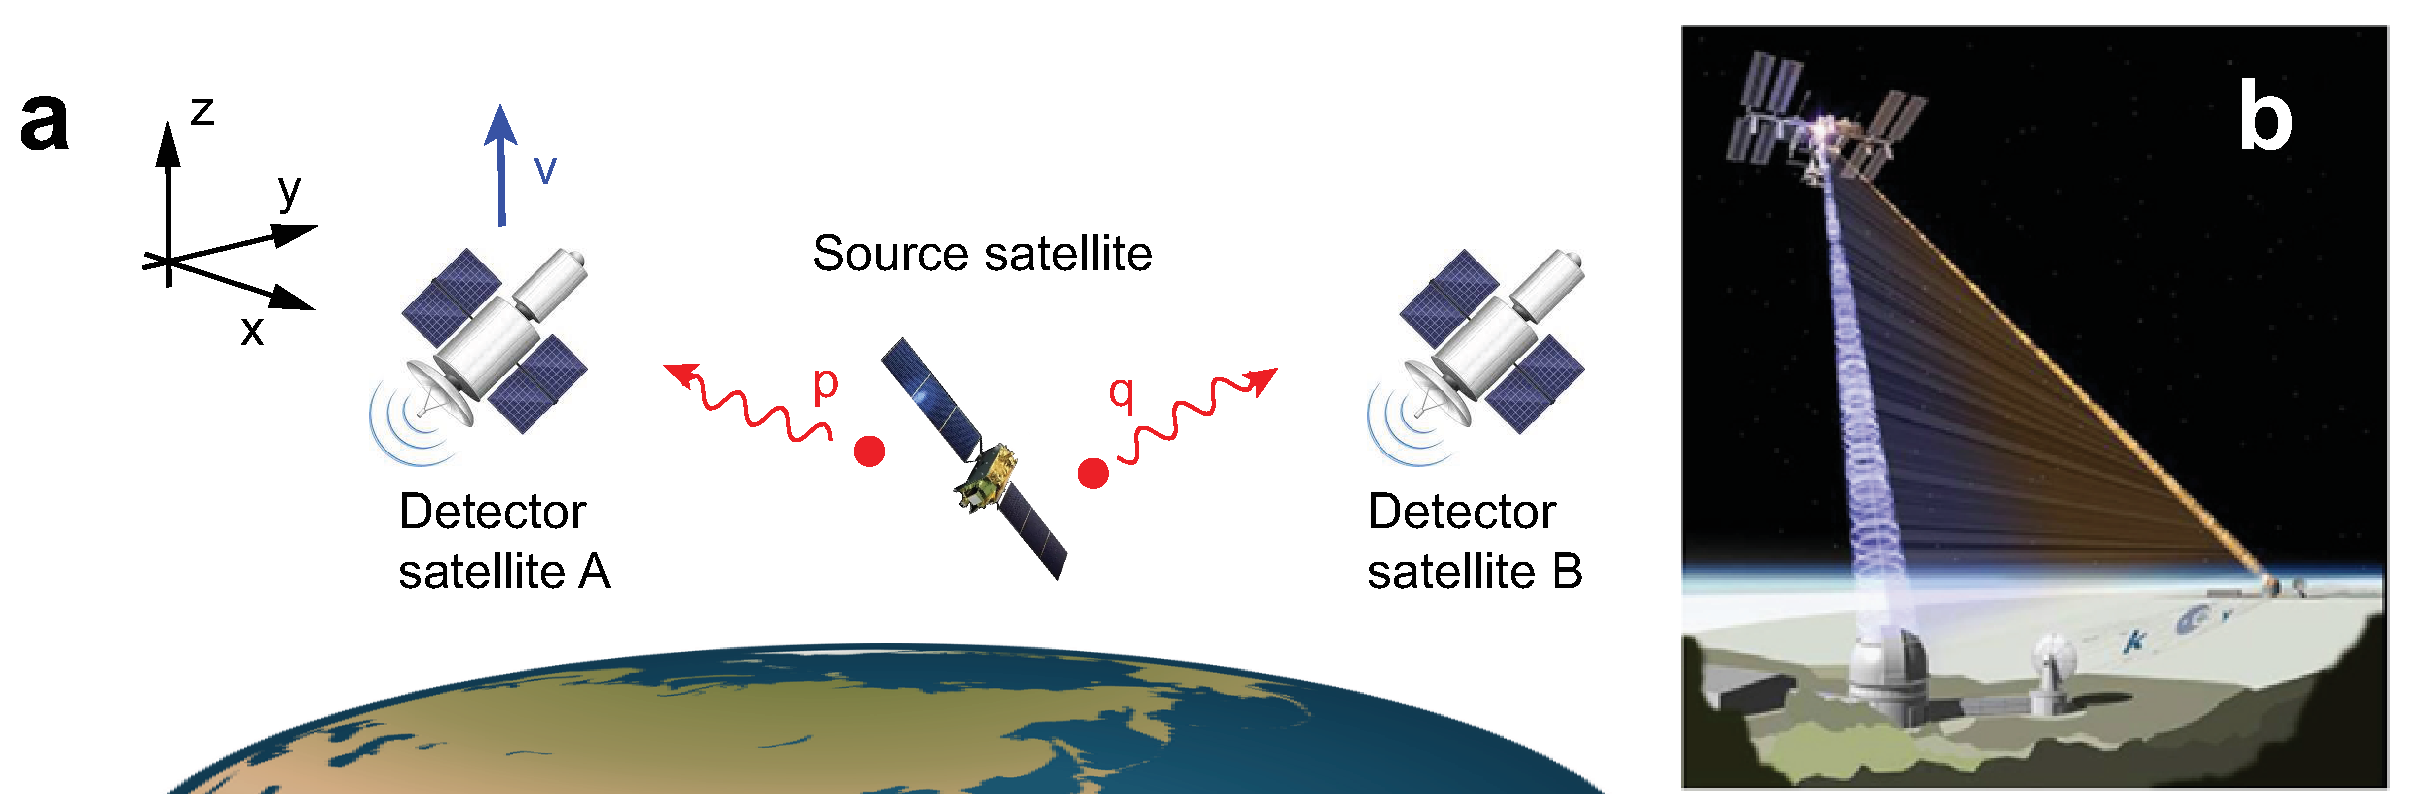
\includegraphics[width=\columnwidth]{figspace1}
\caption{Various possibilities for space-based quantum communication. (a) Satellite-to-satellite quantum communication \cite{byrnes2017lorentz}; (b) Ground-to-satellite quantum communication \cite{armengol08}. }
\label{figspace1}
\end{figure}
















\subsection{International efforts for space-based quantum communication}


\begin{figure*}
\includegraphics[width=2\columnwidth]{figspace4}
\caption{The Chinese Micius quantum communications satellite.  (a) Schematic of the satellite and ground stations used to observe the entangled photons \cite{popkin17}.  [TB: Took image from Science News, may need permission] (b) Attenuation during entanglement distribution from Ref. \cite{yin2017satellite}.  (c) Fidelities achieved for teleportation of various states as marked from Ref. \cite{ren2017ground}.  
}
\label{figspace4}
\end{figure*}




\subsubsection{China: QUESS}

In 2016, the group at the University of Science and Technology led by Jian-Wei Pan launched QUESS (Quantum Science Experiment Satellite), a quantum communication satellite \cite{gibney16,xin11}. The main feature of the satellite is an ultrabright source of polarization entangled photons at 810 nm, generated by parametric down conversion.  The source is capable of emitting $ 5.9 \times 10^6 $ photon pairs per second with a fidelity of $ \sim 0.91 $.  The other important piece of technology is the acquiring, pointing, and tracking technology, which allows the ground stations to track the location of the satellite as it moves across the sky, and vice versa.  This is achieved using lasers at separate wavelengths, and allows the photon transmission and the ground-based receivers to be pointing to each other to within $ \sim 1.2 $ mrad \cite{yin2017satellite}.  The major aims of the project are to perform QKD between Xinglong and Urumqi (a distance of 2500 km); test Bell’s inequality across a distance of 1200 km; and perform teleportation between the satellite and Ali in Tibet (see Fig. \ref{figspace4}).  The final aim is to perform QKD between Beijing and Vienna (a distance of 7500 km). 

At the time of writing three main results have been reported.  The first is an entanglement distribution experiment where a Bell violation was observed between ground stations at Delingha and Lijiang (separated by 1203 km) and Delingha and Urumqi (separated by 1120 km) \cite{yin2017satellite}.  The satellite is in an orbit at a elevation of $ \sim 500$ km, and is in view from the observatories for a duration of $ \sim 275 $ s.
The attenuation of the photons during the downlink transmission is shown in Fig. \ref{figspace4}(b). Taking into account of the distances of the photon transmission, the attenuation rates are far better than the best performance of optical fibers at 0.16 dB/km \cite{yin2013lower} and even theoretical loss limits.  The Bell violation that was recorded in this experiment was at the level of $ 2.37 \pm 0.09 > 2 $, and the nonlocality of the entanglement was confirmed.

The second experiment performed quantum teleportation from the ground to the satellite \cite{ren2017ground}. In the experiment, a single polarization encoded photon defines the qubit to be sent, and the satellite acts as the receiver.  The entangled photons are generated on the ground, at the observatory in Ngari, Tibet. As with the first experiment above, the satellite is in orbit and sweeps across the sky during which the teleportation must be achieved.  The longest distance where the teleportation was successful was at a distance of $ \sim 1400 $ km when the satellite emerges from the horizon.  When directly overhead, the satellite is at a distance of $ \sim 500 $ km.  As Fig.  \ref{figspace4}(c) shows, the fidelity of the types of states teleported are all above the theoretical classical bound of $2/3$, with an average of $ 0.80 \pm 0.01 $.  

A third experiment performed quantum key distribution in a satellite-to-ground configuration, where the ground station was at Xinglong \cite{liao2017satellite}. The protocol that was used is the decoy-state BB84 protocol, which is robust against a photon number splitting attack.  A key rate of between 1 to 12 kbit/s was achieved while the satellite was visible, depending upon the location in the sky (see Fig. \ref{figspace4}(d)).  


















\subsubsection{Japan: SOCRATES}

SOCRATES (Space Optical Communications Research Advanced Technology Satellite) is a microsatellite developed by NICT (National Institute of Information and Communications Technology) \cite{horiuchi2015view,toyoshima2015current,takenaka2017}. This is a $ 48 $ kg satellite with volume $ 50^3 $ cm$^3$ that demonstrates multi-purpose (i.e. both classical and quantum) optical communications. Its main mission is to demonstrate laser communication in space. As one of its subgoals, the on-board equipment is adapted to perform QKD experiments. The satellite is equipped with photon source where the polarization can be changed in non-orthogonal directions.  
Initial results indicated polarization preservation of photons emitted from the satellite, which is a preliminary step towards performing protocols such as BB84 \cite{carrasco2016leo}. More recent results showed quantum limited  satellite-to-ground communication was possible, attaining a quantum bit error rate below 5 \% \cite{takenaka2017} during the closest approach of the satellite to the ground at a distance of $ 744 $ km.  The downlink was established up to distances of over 1000 km, although the error rate was higher for longer distances.  




\subsubsection{Singapore: Cubesat}

The group at the National University of Singapore also has taken the approach using nanosatellites, with the capability of generating correlated photon pairs on-board \cite{tang2016generation}.  
The nanosatellite is 1.65 kg and has the components necessary for creating and detecting parametric down converted photon pairs. The nanosatellite approach greatly reduces the cost for launching into space, and the launch itself was performed by the India’s space agency. As the generation and detection are both on the same satellite, no quantum communication channel (to other satellites or Earth) was established in the experiment, although it showed the space worthiness of the basic quantum optical components. 











\subsubsection{Europe: Retroreflector satellite}

European groups used laser-ranging satellites fitted with corner cube retro-reflectors to demonstrate quantum communication through the atmosphere \cite{villoresi08,vallone15}. A ground based photon source sent up photons towards the satellite, and reflected down again to an Earth based observatory. This showed the ability of photons to travel through the atmosphere into space and back, with a bit error ratio at the level of 5\%. Although no optical sources or detectors were placed on the satellite, there has been long standing active interest in a European space-based quantum communication project, led in particular by the group of Anton Zeilinger at the University of Vienna \cite{armengol08}.  The aims of such projects are to perform space-based QKD, with terrestrial free-space experiments \cite{ursin07,ma2012quantum} as part of the overall effort. 











\subsubsection{Canada: QEYSSat}

The QEYSSat (Quantum EncrYption and Science Satellite) proposes a microsatellite that incorporates a quantum receiver \cite{jennewein2014qeyssat}. The satellite acts as a trusted node, where photons would be transmitted from Earth-based sources. This could be used to perform QKD between two locations on Earth that are separated by large distances. No photon sources or quantum memories would be included on the QEYSSat. 





\begin{figure}
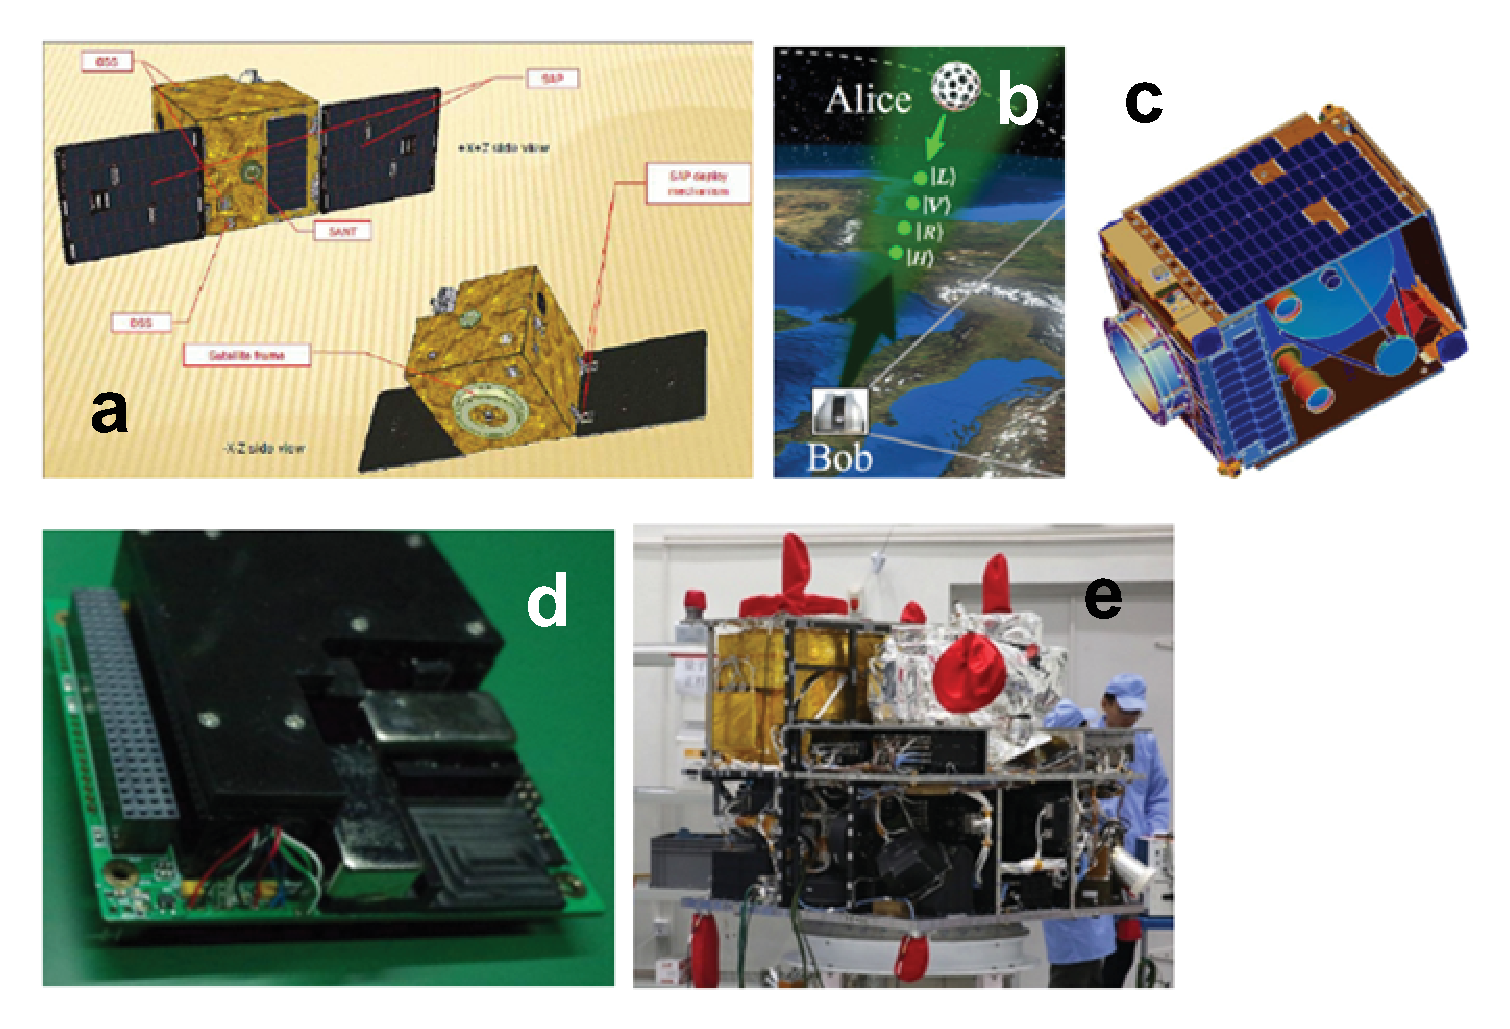
\includegraphics[width=\columnwidth]{figspace2}
\caption{Satellites employing quantum technologies from various groups across the world: Japan \cite{horiuchi2015view}, Italy \cite{vallone15}, Canada \cite{jennewein2014qeyssat}, Singapore \cite{tang2016generation}, and China \cite{gibney16}.}
\label{figspace2}
\end{figure}









\subsection{Applications of a space-based quantum network}

\subsubsection{Quantum key distribution}

As we have discussed in Sec. [TB:please fill this in], the demand for secure cryptography is now extremely important in the context of electronic commerce and general security of information transmission in the internet age. Electronic currencies such as Bitcoin depend on cryptographic protocols in order to secure the value of the assets, assign ownership, and secure the currency against fraud.  However such protocols are based upon computational complexity of certain mathematical problems, and are not fundamentally secure in the presence of limitless computational resources, or quantum computers.  Therefore, using quantum mechanical protocols which are based on physical principles rather than computational limitations, are favorable in the sense of future-proofing the security.  Quantum key distribution is a relatively mature technology with already several commercial systems being available.  The main drawback is thus the ability to perform long-distance transmission of photons.  For these reasons, current quantum key distribution networks have been limited relatively small area in the region of $ \sim $ 100 km, such as in Austria, Switzerland, Japan, USA, and China \cite{lo2014secure}.   The longest distance QKD network that is currently planned is the Beijing to Shanghai quantum key distribution link spanning a distance of 2000 km.  This involves 32 trusted nodes to break the total distance into shorter segments to convert the quantum information to classical information.  

Utilizing space communications for the purpose of quantum key distribution has been discussed in several works \cite{hughes2000quantum,rarity2002ground,pfennigbauer2003free,aspelmeyer2003long,armengol08}. As already demonstrated in the space entanglement  experiments \cite{yin2017satellite,ren2017ground,liao2017satellite} far lower attenuation rates are possible using the technique that in either free space or optical fiber methods.  Since cryptography schemes such as BB84 do not require entanglement, these would appear to be the first commercial widespread application of quantum technologies.  The high feasibility of space based quantum key distribution was already noted in a variety of configurations including ground-to-space and space-to-ground quantum communication \cite{rarity2002ground,aspelmeyer2003long}.  In the context of security, the first long-distance experiments that are likely to be performed employing trusted nodes.  For example, after performing quantum key distribution between satellite and a ground station, a satellite could store the key for some time until another quantum key distribution can be performed to another ground station using a one-time pad \cite{liao2017satellite}.  These types of experiments are planned eventually to perform intercontinental quantum key distribution between China and Austria.  









\subsubsection{Quantum clock synchronization}


Clock synchronization is a fundamental task that is has widespread applications, ranging from navigation, telecommunications, financial transactions, the internet, and many scientific applications. Of these, the Global Positioning System (GPS) has become a day-to-day necessity for a large fraction of the human population as it has been increasingly built into smartphones and other devices. The GPS system famously relies upon very precise clock synchronization to perform its task through a process of quadrangulation from several satellites. Due to the high speed of light, one requires in practice highly synchronized clocks which are accurate to a centralized time standard to the $\sim$ ns level. This allows positioning to be performed to the $\sim$ m level, which is acceptable for many applications. GPS satellites have atomic clocks that are stable to one part in $10^{13}$, so that active corrections can maintain the accurate to the $\sim$ ns level. The great success of the GPS system in turn has created a further demand for increasingly precise navigation. For example, autonomous vehicles would immediately benefit from a more precise navigation system. In principle, technology for more stable clocks is already present, with atomic clocks exceeding stabilities of those on satellites being routinely produced, and optical atomic clocks now reaching stabilities of one part in $10^{18}$  \cite{ludlow2015optical}. An outstanding question is then how to synchronize these clocks given their remarkable stabilities. 


\begin{figure}
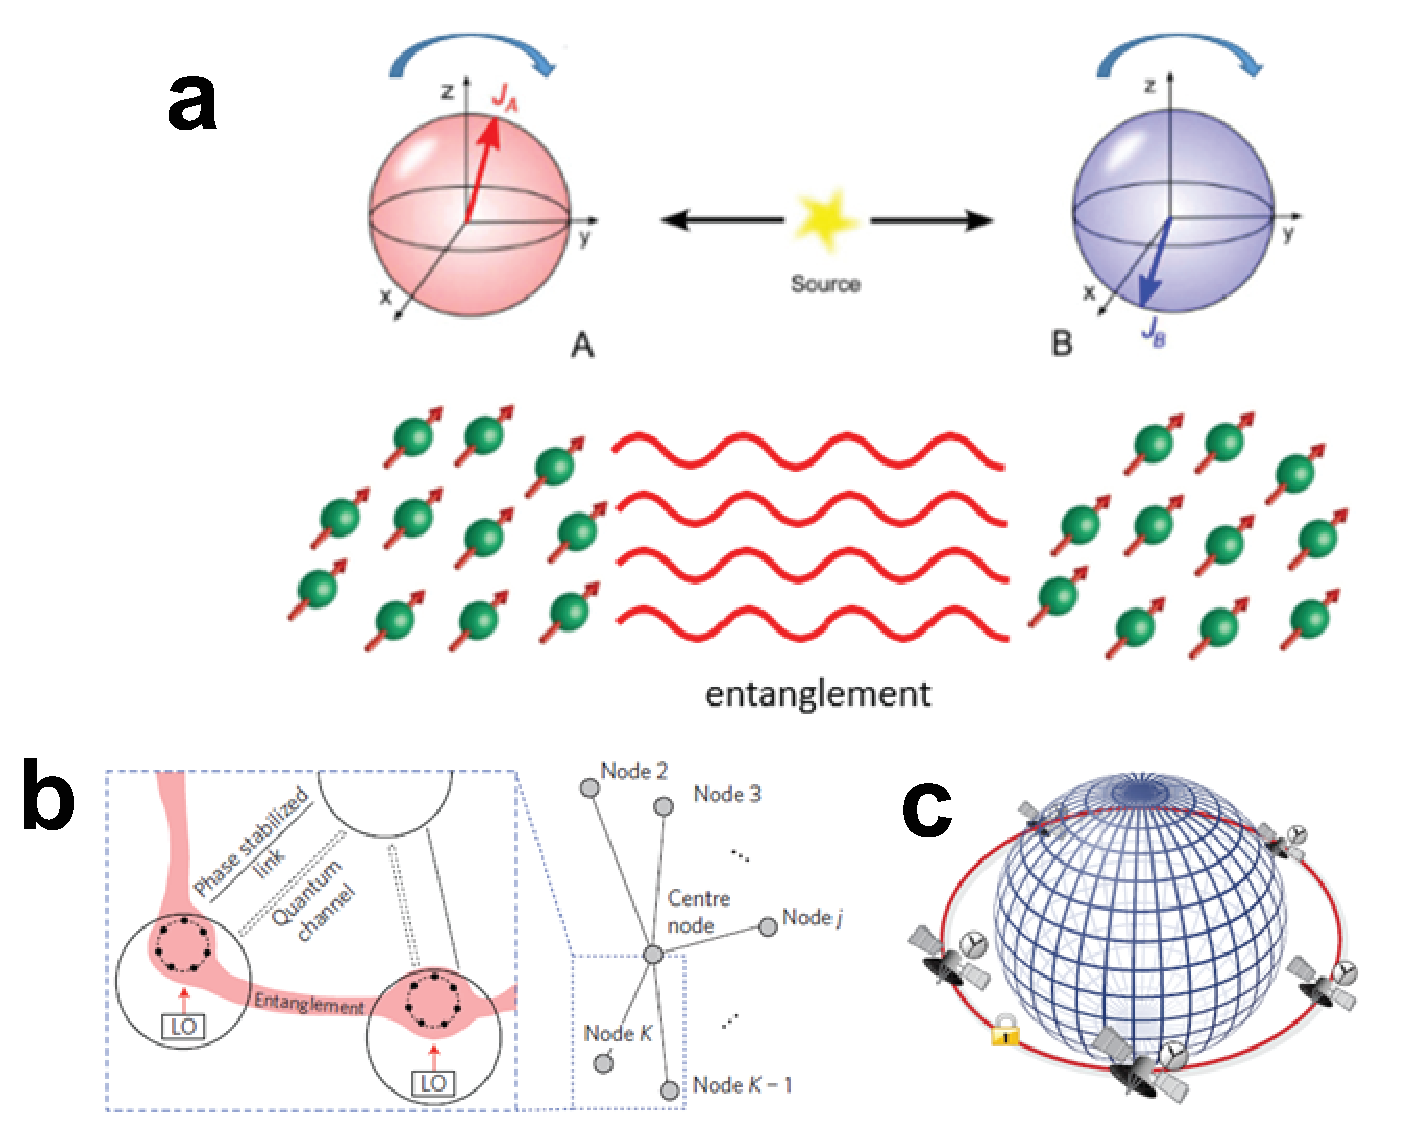
\includegraphics[width=\columnwidth]{figspace3}
\caption{Quantum clock synchronization schemes. (top) The proposal by Jozsa, Dowling, and co-workers where a singlet state is shared and measured in an ensemble of qubits \cite{jozsa00}. (bottom) The proposal by Lukin, Ye, and co-workers where a GHZ state is generated between satellites to obtain measure the frequency drift at the Heisenberg limit \cite{komar14}. }
\label{figspace3}
\end{figure}



Several past works have examined the problem of clock synchronization in space (see also Sec. [TB: refer to other section on clock sync]). In the proposal of Jozsa and co-workers, many copies of shared entanglement in a singlet state is first distributed and stored on the clock states of an atomic clock \cite{jozsa00}.  The measurement is then made by one of the parties, which collapses the states simultaneously at each party, and the time evolution of the states begins. Classical information is exchanged between them, which reveals the time elapsed since the measurement, which can be used to synchronize the clocks. While the original protocol only allowed allowed clock synchronization between two parties, similar ideas were used to extend it to a multiparty context \cite{krvco2002quantum,ben2011optimized,ren2012clock}.  In a more recent proposal, a shared GHZ state is prepared across all the nodes of the quantum network, which allows for a quantum metrologically enhanced detection of the clock signal drift at the Heisenberg limit \cite{komar14}. The use of shared resources acts to improve the overall precision, allowing for an optimal scheme for the qubit resources that are used. Several other proposals have also been made, which are quantum versions of Eddington's slow clock transport where the qubit keeps time of the transmission time \cite{chuang2000quantum,tavakoli2015quantum}. 

Experimentally, there have been several demonstrations of the protocol, albeit at relatively short distances.  Continuous time-bin entangled photons were used as the entanglement resource to obtain a time-correlation between a distance of 3 km \cite{valencia2004distant}, and another technique based on Hong-Ou-Mandel interferometry was performed with a 4 km fiber link \cite{quan2016demonstration}.  Several other demonstrations based on NMR \cite{zhang2004nuclear,kong2017implementation} have also been performed. 

There are however several outstanding problems with the quantum clock synchronization scheme as presented above. In the scheme of Jozsa and co-workers, if one starts in a perfect singlet state, the scheme works as intended, but if one instead starts in the state 
%
\begin{align}
\frac{1}{\sqrt{2}} \left( | 0 \rangle_A | 1 \rangle_B - e^{i \delta} | 1 \rangle_A | 0 \rangle_B \right)
\end{align}
%
then one obtains an offset to the synchronizations between the two parties. In practice, such a phase could arise from decoherence induced noise, or differences in the basis conventions that the two parties choose. Thus in practice entanglement purification would to be performed to produce a singlet state with $ \delta = 0 $ before the synchronization protocol is performed.  However, it was argued that to perform the entanglement purification quantum circuit correctly, the timing of the quantum gates would need to be controlled, which requires synchronized clocks \cite{preskill2000quantum} --  rendering the syncrhonization impossible. It was previously been shown that such a phase cannot be eliminated using asynchronous entanglement purification \cite{yurtsever02}, and hence the protocol remains incomplete in the general case where imperfect singlet pairs are shared. 








\subsubsection{Fundamental physics experiments}

The availability of a globe-spanning quantum network on satellites brings the opportunity for fundamental quantum mechanical experiments and unprecedented length scales and velocities in the future.  Satellite-to-satellite photon transfer can allow for ultra-long distance quantum communications that are not possible on Earth due to atomospheric loss.  Another unique aspect of space is that the satellites are moving at high velocity –- typically at $10^{-5} $ times the speed of light for low Earth orbit satellites.  The combination of both of these effects gives a unique opportunity for performing relativistic quantum information experiments to test fundamental physics. 

We anticipate that some of the first choices of experiments will be extensions of what are already performed on Earth.  For example, one can perform increasingly long space-based Bell violation tests at unprecedented distances \cite{yin2017satellite}.  Another possibility is to examine the speed of influence of entanglement, which bound the speed of entanglement \cite{yin2013lower}.  In space, such experiments could be extended much further, giving tighter bounds.  There are demanding technical hurdles that must be overcome to accomplish such experiments, such as the necessity of synchronized clocks. In addition to examining extensions of existing experiments, the high satellite velocities can be used to perform relativistic quantum information experiments, such as entanglement tests in the presence of special and general relativity, Wheeler's delayed choice experiment, and enhanced quantum metrology \cite{kaltenbaek2003proof,scheidl2013quantum,ahmadi2014relativistic}.  












\subsection{Future challenges}

\subsubsection{Coverage}

Currently there are only two satellites with capability of sending and/or receiving photons through space, the Chinese QUESS and the Japanese SOCRATES satellites.  In order to achieve world-wide coverage multiple satellites would be necessary such that there would be a constellation of satellites that are visible at all times, anywhere on Earth, in a similar way to GPS satellites. In the case of the QUESS satellite, the orbit is such that it passes over the observatories once per day, with a visibility window of $ \sim 275 $ s.  The coverage of a low Earth orbit satellite of elevation 500 km has a maximum radius of $ \sim 2400 $ km from the point where the satellite is directly overhead due to the curvature of the Earth.  In practice it will be less than this due to obstacles and due to atmospheric influence, which reduce it to distances of the order of $ \sim 1000 $ km (see Fig. \ref{figspace4}). By launching satellites at higher orbits, it will be possible to increase the coverage, which will lead to extra challenges in establishing a satellite link.  Some of the technologies that will need to be developed are larger-size telescopes, better tracking systems, and wave-front correction through adaptive optics \cite{liao2017satellite}.  Currently the communications are performed at night due to the laser wavelengths that are used, but plans for using telecommunication wavelengths give the possibility of daytime quantum communication. 


From the point of view of security, we anticipate that the initial quantum networks for quantum key distribution will be based on trusted nodes.  Due to the difficulty of tampering of space-based trusted nodes, it is likely that this will offer a sufficient level of security for most applications. Thus using a constellation of satellites employing quantum key distribution can achieve long-distance cryptography by simply relaying the information, either by multiple satellite-to-ground or a satellite-to-satellite configuration.  For the ultimate security without the use of trusted nodes, one would employ alternative protocols that do not require line-of-sight quantum communication, such as the E91 protocol \cite{ekert1991quantum}.  As this requires entanglement distribution, storage, and purification, this would be most likely a second generation technology after the trusted node quantum key distribution network is already established.   








\subsubsection{High precision applications}

For applications such as quantum clock synchronization and fundamental experiments testing physics at large length scales and velocities, it is likely that extremely high fidelities of the quantum operations will be necessary.  For example, for clock synchronization, even current atomic clocks used as national standards have an accuracy at the level of $ 10^{-14} $.  Thus such high precision experiments will almost certainly follow the less demanding quantum key distribution experiments.  As the precision of the technology improves, other sources of error may appear which may require correction.  It is well-known from existing GPS satellites, it is crucial to account for relativistic effects, due to time-dilation and the gravitational red shift. Not accounting for these effects would seriously compromise the GPS system, with inaccuracies equating to an error of the order of 10 km/day. This is due to the high velocities of LEO satellites, traveling at speeds of  $ \beta = 10^{-5} $ times the speed of light. Such relativistic effects can affect the entanglement in the presence of diffracting photons \cite{gingrich03}.  Even for single photon transmission, polarization encoded photons can give rise to correction at the order of $ \beta $ \cite{byrnes2017lorentz}.  Using relativistically invariant entanglement distribution protocols have been proposed by several authors to avoid such effects, which would otherwise require correction \cite{yurtsever02,li2003relativistic,byrnes2017lorentz}.  

















\section{Conclusions}
\label{conclusions}


[Conclusions]






\section{Acknowledgments}
T. B. is supported by the Shanghai Research Challenge Fund; New York University Global Seed Grants for Collaborative Research; National Natural Science Foundation of China (Grant No. 61571301); the Thousand Talents Program for Distinguished Young Scholars (Grant No. D1210036A); and the NSFC Research Fund for International Young Scientists (Grant No. 11650110425); NYU-ECNU Institute of Physics at NYU Shanghai; and the Science and Technology Commission of Shanghai Municipality (Grant No. 17ZR1443600). 

J. P. D. would like to acknowledge support from the US Air Force Office of Scientific Research, the Army Research Office, the National Science Foundation, and the Northrop-Grumman Corporation.  



\bibliography{references}

\end{document}
